\documentclass[11pt,a4paper]{article}
\usepackage[utf8]{inputenc}
\usepackage[T1]{fontenc}
\usepackage[french]{babel}
\usepackage{amsmath, amssymb}
\usepackage[margin=2.5cm]{geometry}
\usepackage{graphicx}
\usepackage{hyperref}
\usepackage{titlesec}
\usepackage{parskip}

%\titleformat{\section}{\large\bfseries}{\thesection}{1em}{}
%\titleformat{\subsection}{\normalsize\bfseries}{\thesubsection}{1em}{}

\title{Hyperpop! \\ \normalsize{Jeu de tir sur des sphères 4D}}
\author{Caio COSTA, Youssef SAIDI}
\date{Printemps 2025}

\begin{document}

\maketitle

\tableofcontents

\section{Introduction}

Ce projet a consisté à concevoir un jeu interactif prenant place dans un espace à quatre dimensions, dans lequel le joueur doit tirer sur des sphères 4D. L'originalité du jeu réside dans le fait que l'on ne visualise pas directement les objets 4D, mais uniquement leur intersection avec un hyperplan 3D, que l'on peut déplacer le long de la quatrième dimension.

Ce travail nous a permis d'explorer les concepts de géométrie en dimension supérieure, tout en les rendant accessibles grâce à une représentation tridimensionnelle interactive et intuitive.

\section{Modélisation géométrique}

\subsection{Sphères en 4D}

Une sphère dans un espace à quatre dimensions est définie comme l'ensemble des points de $\mathbb{R}^4$ situés à une distance constante $r$ d'un centre $(x_0, y_0, z_0, w_0)$ :
\[
(x - x_0)^2 + (y - y_0)^2 + (z - z_0)^2 + (w - w_0)^2 = r^2.
\]

\subsection{Hyperplan 3D de visualisation}

Pour visualiser les objets 4D, nous utilisons un hyperplan de la forme $w = c$, avec $c$ variable. Ce plan joue le rôle d’une “caméra” 3D balayant l’espace 4D, et permet d’en extraire une coupe tridimensionnelle observable à l’écran.

Pour comprendre le concept, il est utile de se représenter ce que c'est l'intersection avec un hyperplan en 3D. Donc juste avec un plan, on peut voir que l'intersection avec un cube va donner soit un point, soit un triangle, soit un carré, soit un hexagone, alors qu'avec une sphère ça donne simplement un cercle. Le même concept reste vrai en 4D donc on a décidé de partir sur un jeu avec des sphères 4D.

\begin{figure}[h]
    \centering
    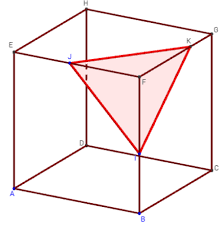
\includegraphics[width=0.3\linewidth]{intersection-cube}
    \caption{Intersection plan cube}
    \label{fig:inter-plan-cube}
\end{figure}
\begin{figure}
    \centering
    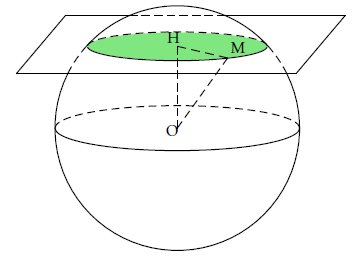
\includegraphics[width=0.3\linewidth]{intersection-sphere}
    \caption{Intersection plan sphère}
    \label{fig:inter-plan-sphere}
\end{figure}

\subsection{Intersection sphère 4D / hyperplan 3D}

L’intersection d’une sphère 4D avec le plan $w = c$ est une sphère 3D (ou vide si le plan est trop éloigné du centre en dimension $w$). Son rayon est donné par :
\[
r' = \sqrt{r^2 - (w_0 - c)^2}
\]
à condition que $|w_0 - c| \leq r$.

\section{Mécanique du jeu}

\subsection{Navigation dans la quatrième dimension}

L’ensemble des objets du jeu est affecté par une matrice \textit{model} représentant leur position dans l’espace. Pour simuler une caméra mobile dans l’espace 4D, on applique à cette matrice des transformations inverses (translations, rotations), déclenchées par les touches pressées par le joueur.

Le joueur peut se déplacer dans l'espace 3D mais également faire déplacer l'hyperplan 3D dans l'espace 4D pour faire apparaître de nouveaux objets.

\subsection{Déplacement des sphères}

Chaque sphère se déplace de manière périodique selon une direction choisie aléatoirement à son apparition. Cela permet de créer une dynamique dans l’espace et de rendre le jeu plus vivant.

\subsection{Système de tir}

Le joueur dispose d’un viseur fixe, situé au centre de l’écran, et peut tirer sur les sphères visibles. Selon la sphère touchée, il obtient un certain nombre de points, et un effet sonore spécifique est joué pour indiquer un tir réussi.

\section{Affichage et rendu}

\subsection{Chunks}

Afin de gérer efficacement l’affichage dans un espace potentiellement très grand, nous avons découpé l’univers en ``chunks'', c’est-à-dire en sous-espaces 3D localisés. Seuls les chunks proches de la position courante du joueur sont affichés.

\subsection{Mise à jour à chaque frame}

À chaque image (frame), le moteur de jeu effectue les opérations suivantes :
\begin{itemize}
    \item Détection des touches pressées et mise à jour de la matrice \textit{model}.
    \item Mise à jour des chunks visibles selon la position du joueur.
    \item Affichage des étoiles et du fond spatial.
    \item Mise à jour de la position des sphères et affichage de leur intersection avec l’hyperplan courant.
\end{itemize}

\subsection{Rendu visuel}

Le rendu est assuré par p5.js. Les sphères issues des intersections 4D–3D sont représentées sous forme de sphères classiques 3D. Le tout est affiché sur fond sombre avec quelques étoiles pour renforcer l’immersion spatiale.

\section{Conclusion}

Ce projet a été l’occasion d’aborder de manière ludique et concrète les défis de la visualisation en dimension supérieure. Il nous a permis de combiner des compétences en géométrie, en programmation graphique et en conception interactive pour créer une expérience originale et pédagogique.


\end{document}
